\chapter{Исследовательская часть}

В данном разделе будет проведено обучение модели гауссовой смеси и сравнение с исходным набором данных.

\section{Предобработка исходных данных}

В качестве набора данных для обучения модели гауссовой смеси были проведены измерения мощности сигнала между источником и приёмником, взаимодействующими по протоколу BLE, на расстояниях от 0.1 до 5 метров. На рисунках \ref{fig:heatmap}-\ref{fig:hist-filtered} представлена визуализация результатов измерений до и после фильтрации.

\begin{figure}[H]
	\centering
	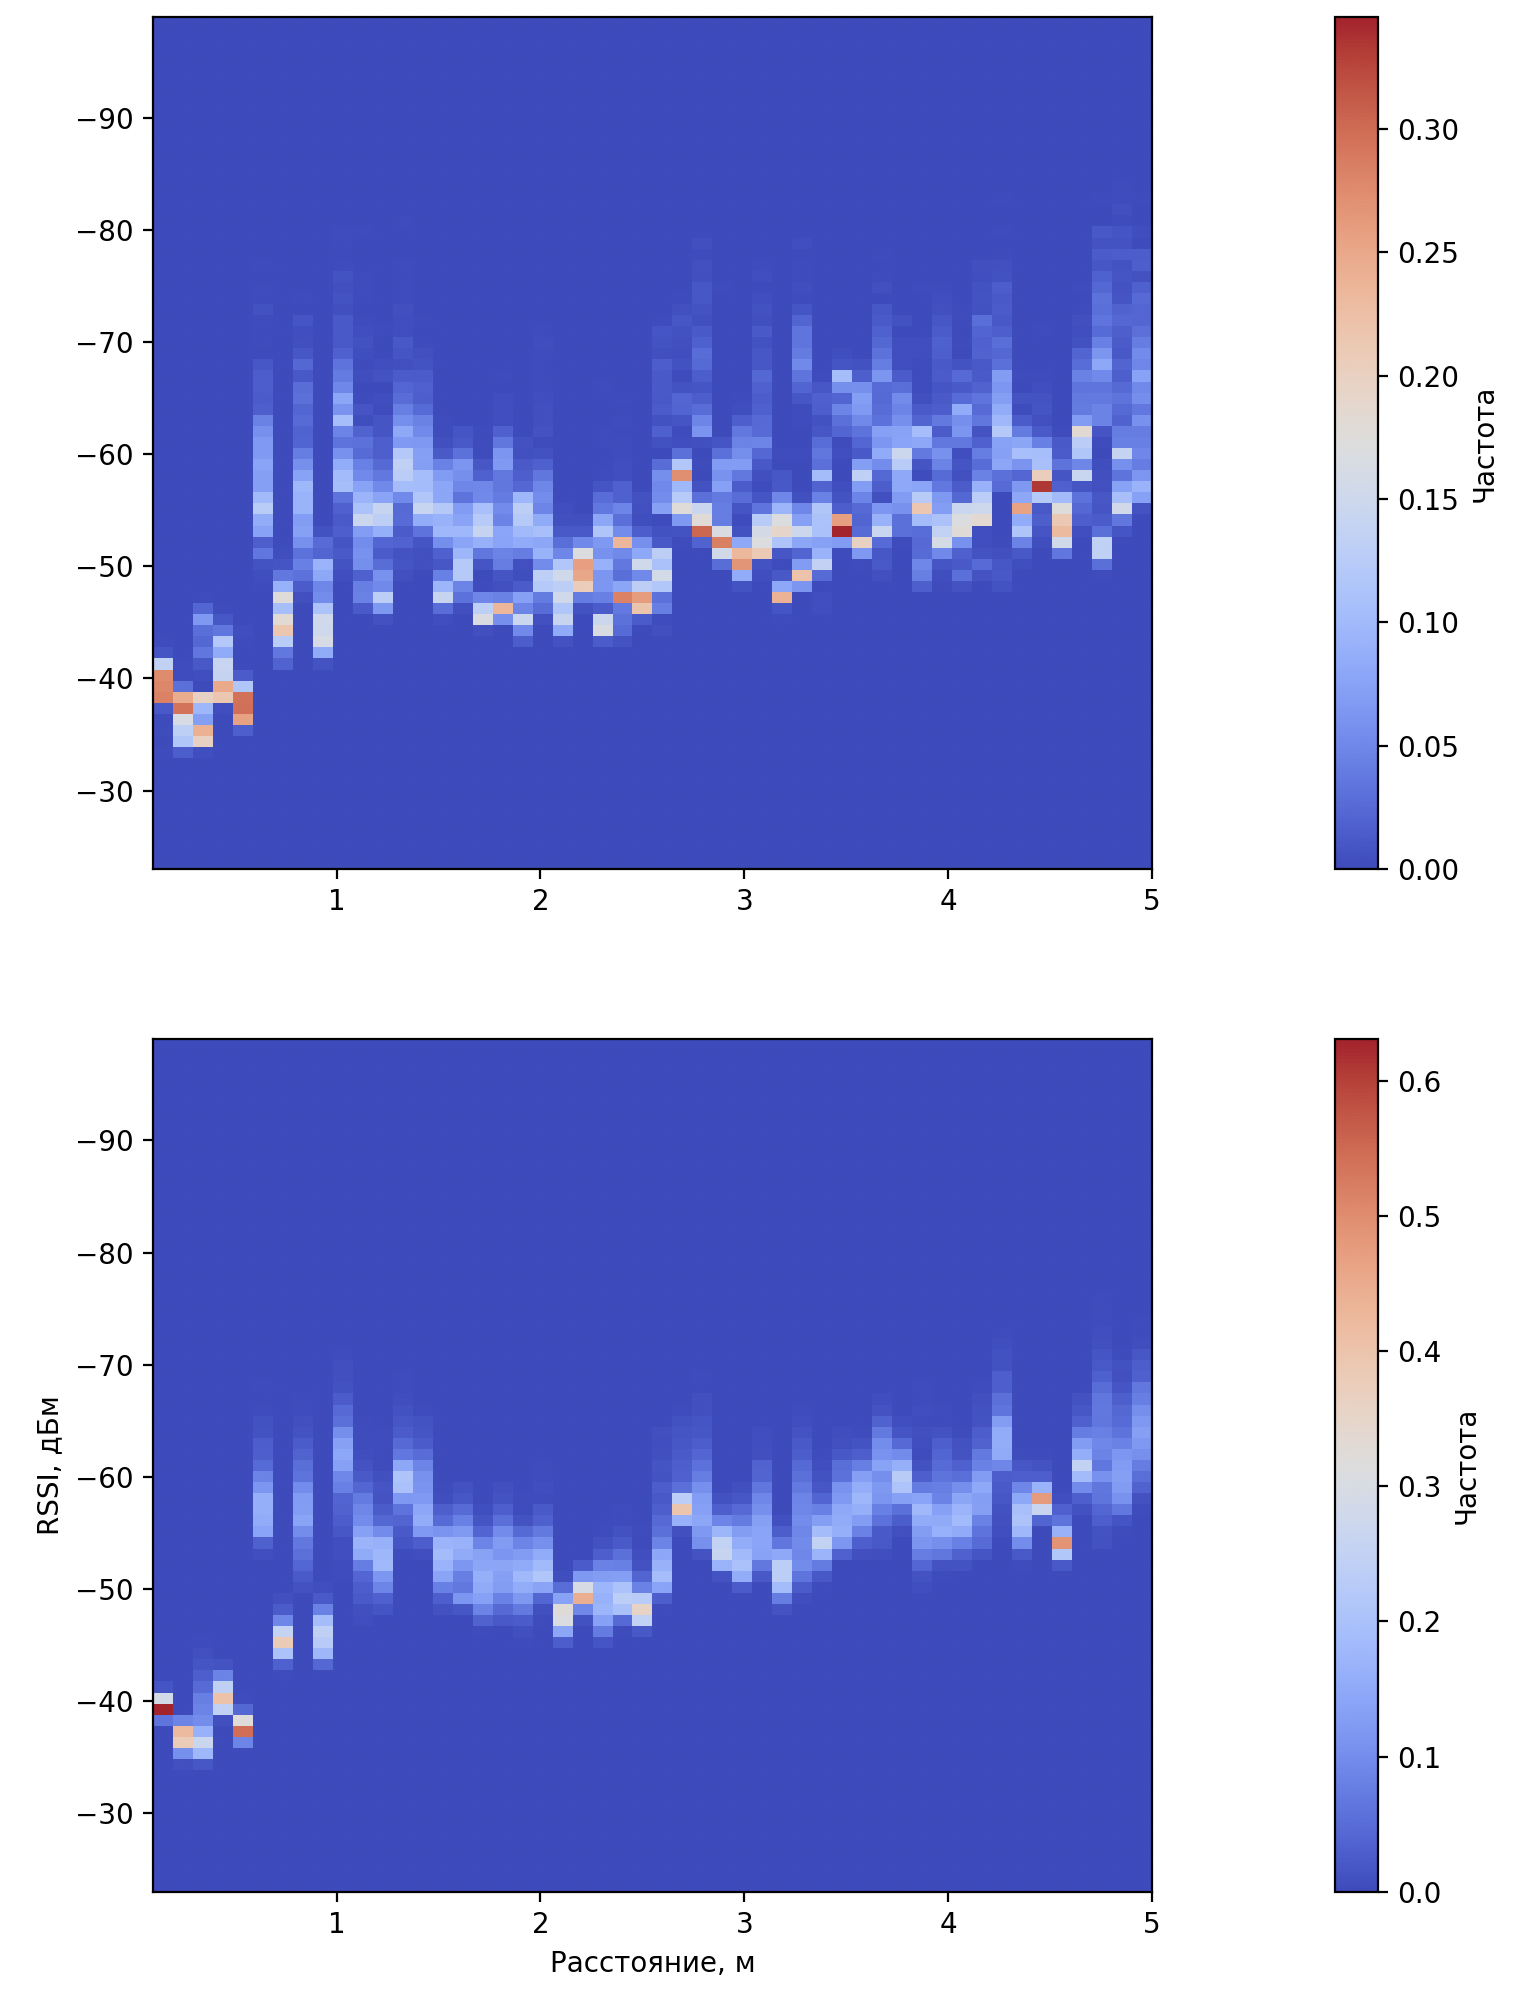
\includegraphics[width=\textwidth]{assets/heatmap.png}
	\caption{Тепловые карты, составленные по датасету до фильтрации (сверху) и после неё (снизу)}
	\label{fig:heatmap}
\end{figure}

\begin{figure}[H]
	\centering
	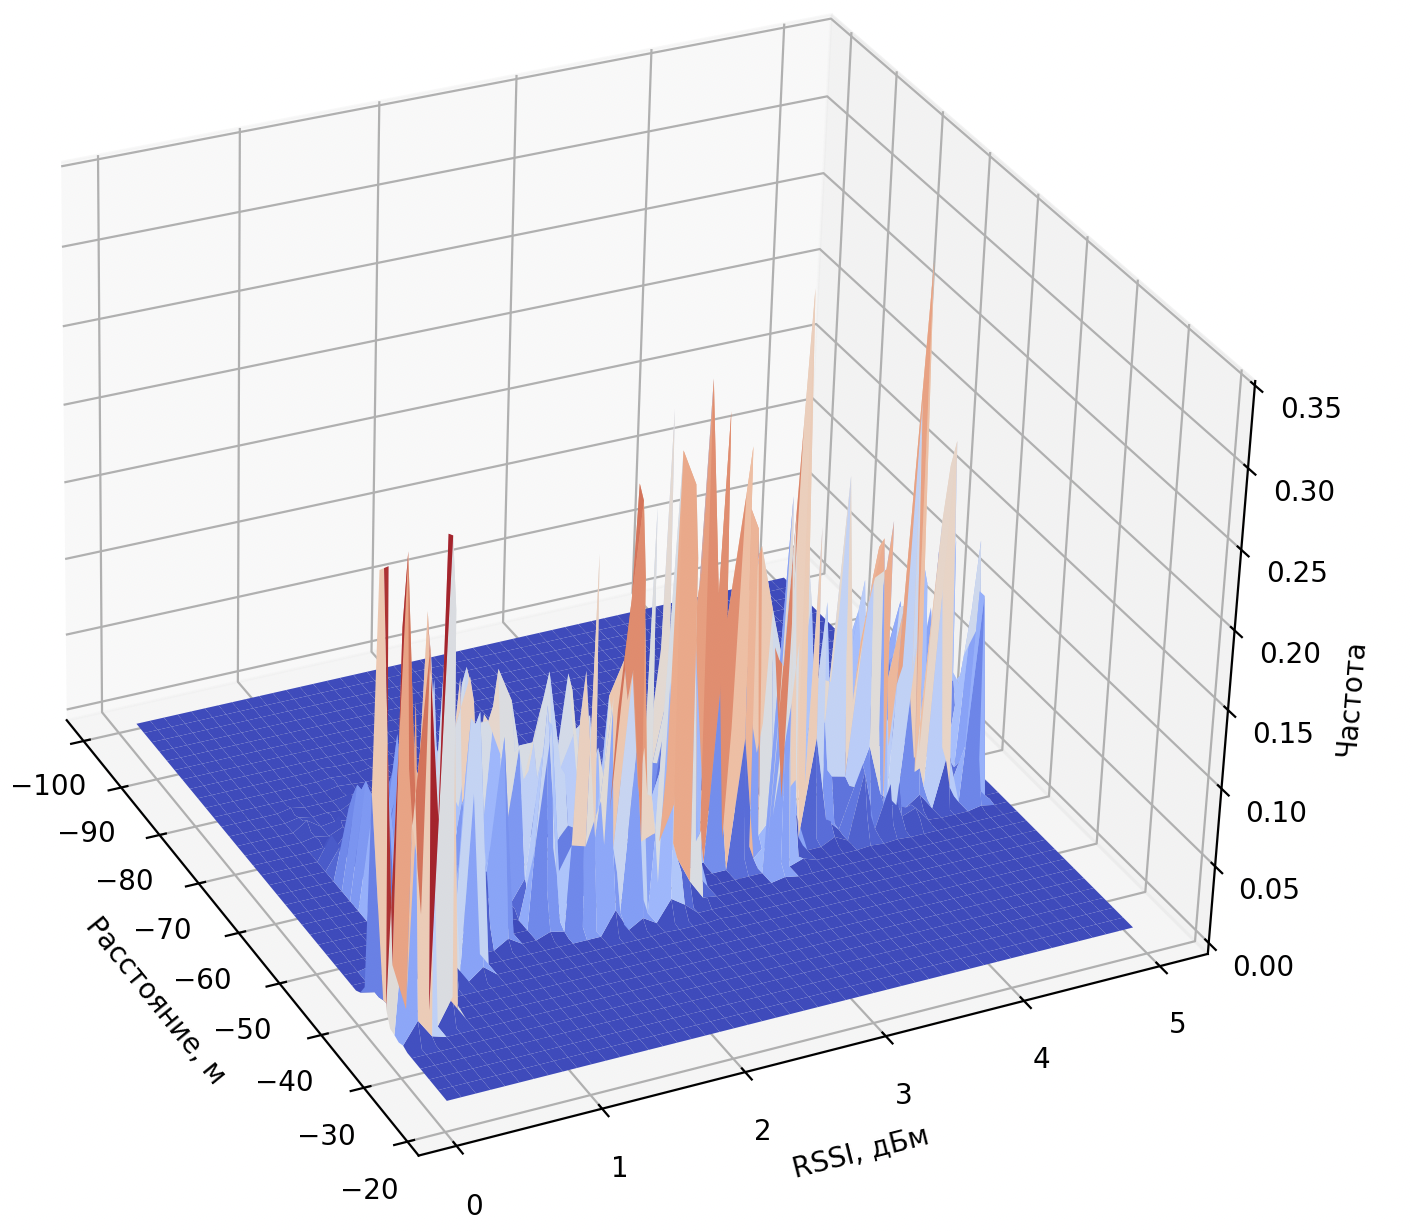
\includegraphics[width=\textwidth]{assets/hist.png}
	\caption{Гистограмма распределения мощности сигнала в зависимости от расстояния между источником и приёмником до фильтрации}
	\label{fig:hist}
\end{figure}

\begin{figure}[H]
	\centering
	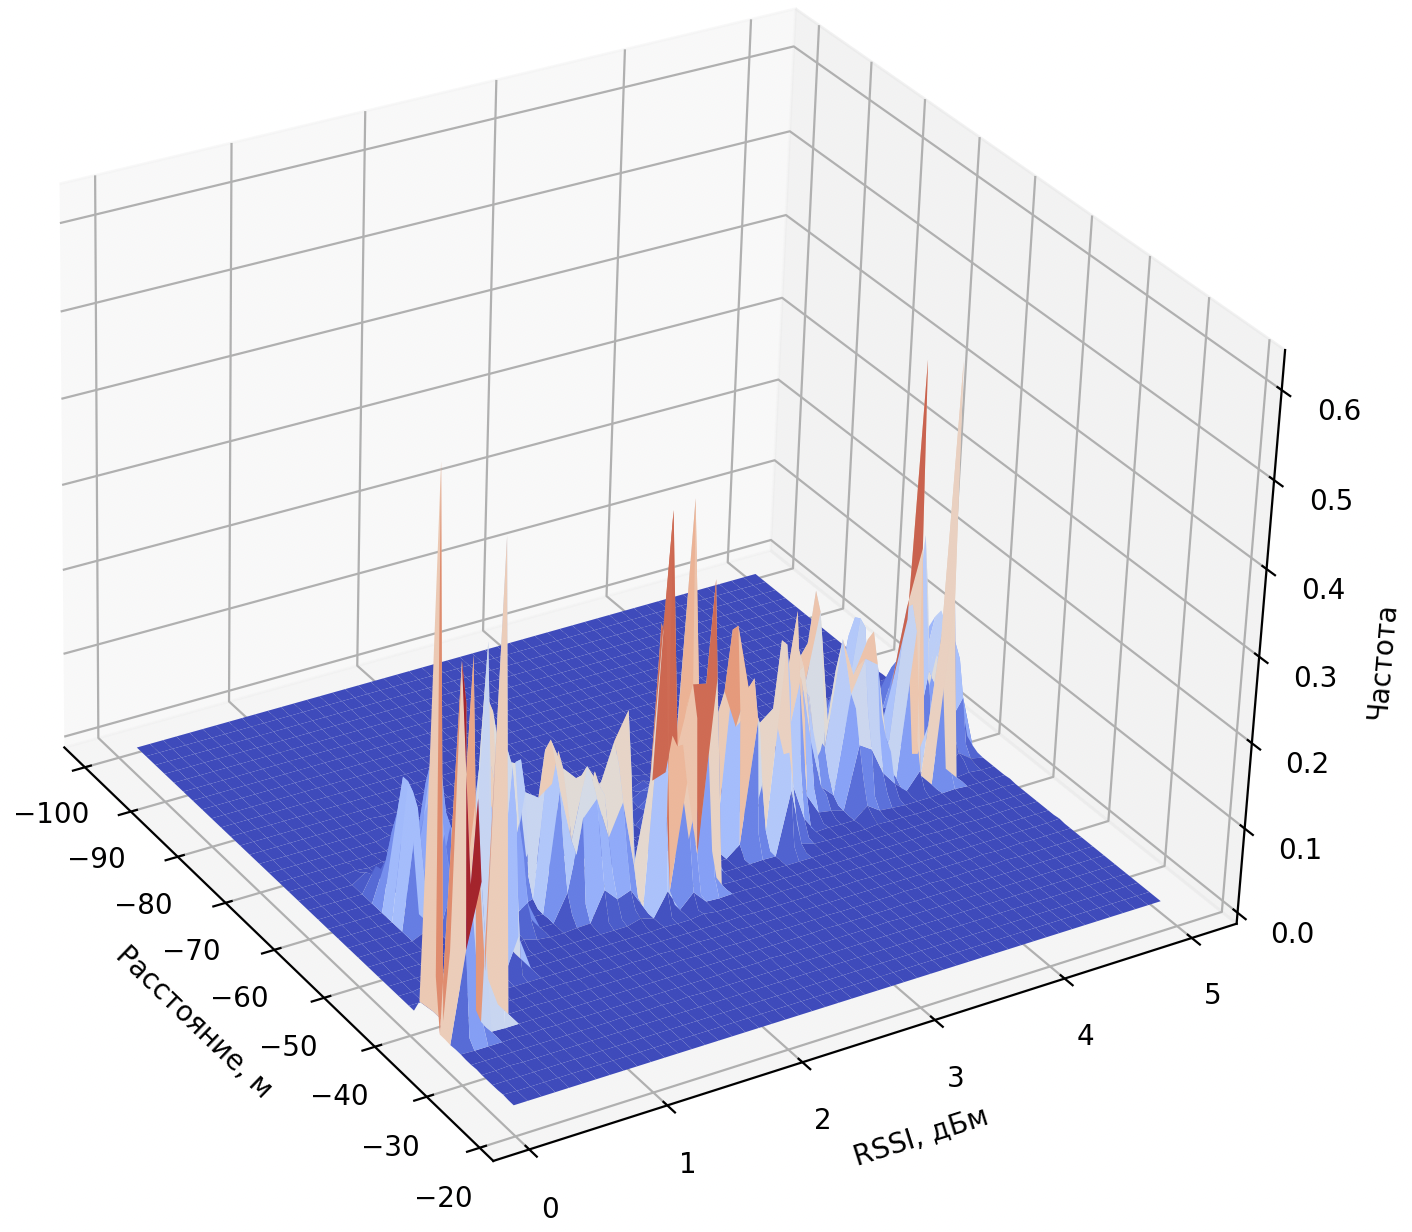
\includegraphics[width=\textwidth]{assets/hist-filtered.png}
	\caption{Гистограмма распределения мощности сигнала в зависимости от расстояния между источником и приёмником после фильтрации}
	\label{fig:hist-filtered}
\end{figure}

На рисунках \ref{fig:means} и \ref{fig:medians} представлено сравнение средних и медианных значений мощности сигнала, а также их отклонений,  до и после фильтрации. Сравнение показывает, что применение фильтра Калмана позволило снизить отклонения мощности сигнала, не изменив при этом средние и медианные значения.

\begin{figure}[H]
	\centering
	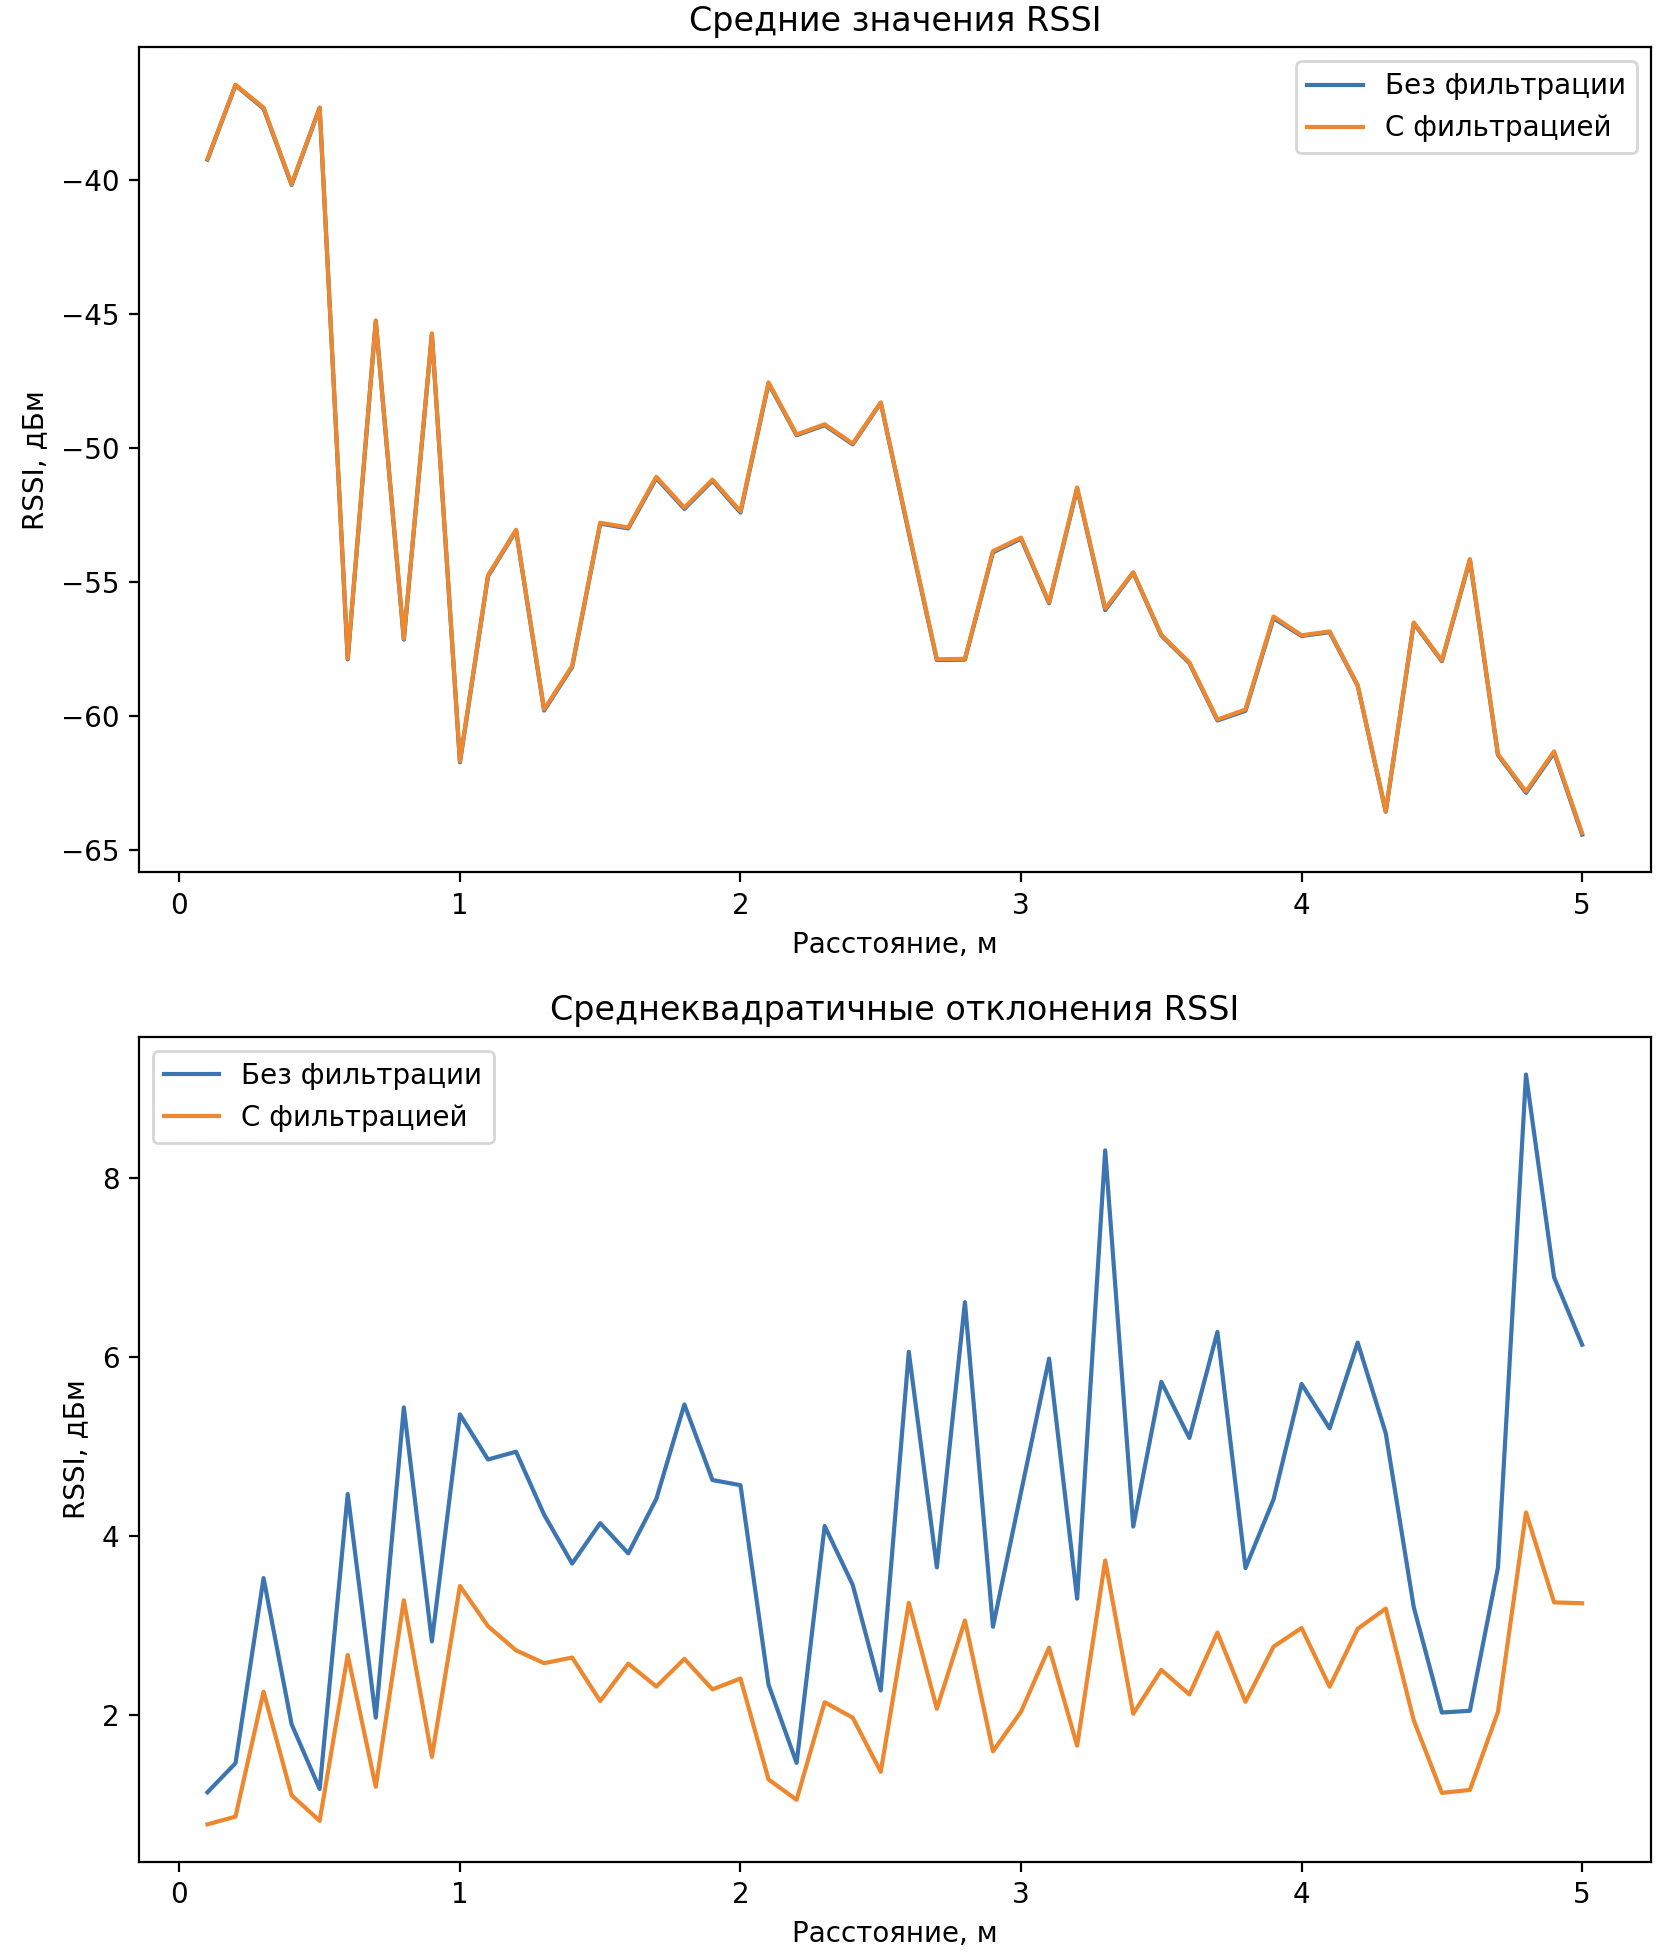
\includegraphics[width=\textwidth]{assets/means.png}
	\caption{Сравнение средних значений мощности сигнала до и после фильтрации}
	\label{fig:means}
\end{figure}

\begin{figure}[H]
	\centering
	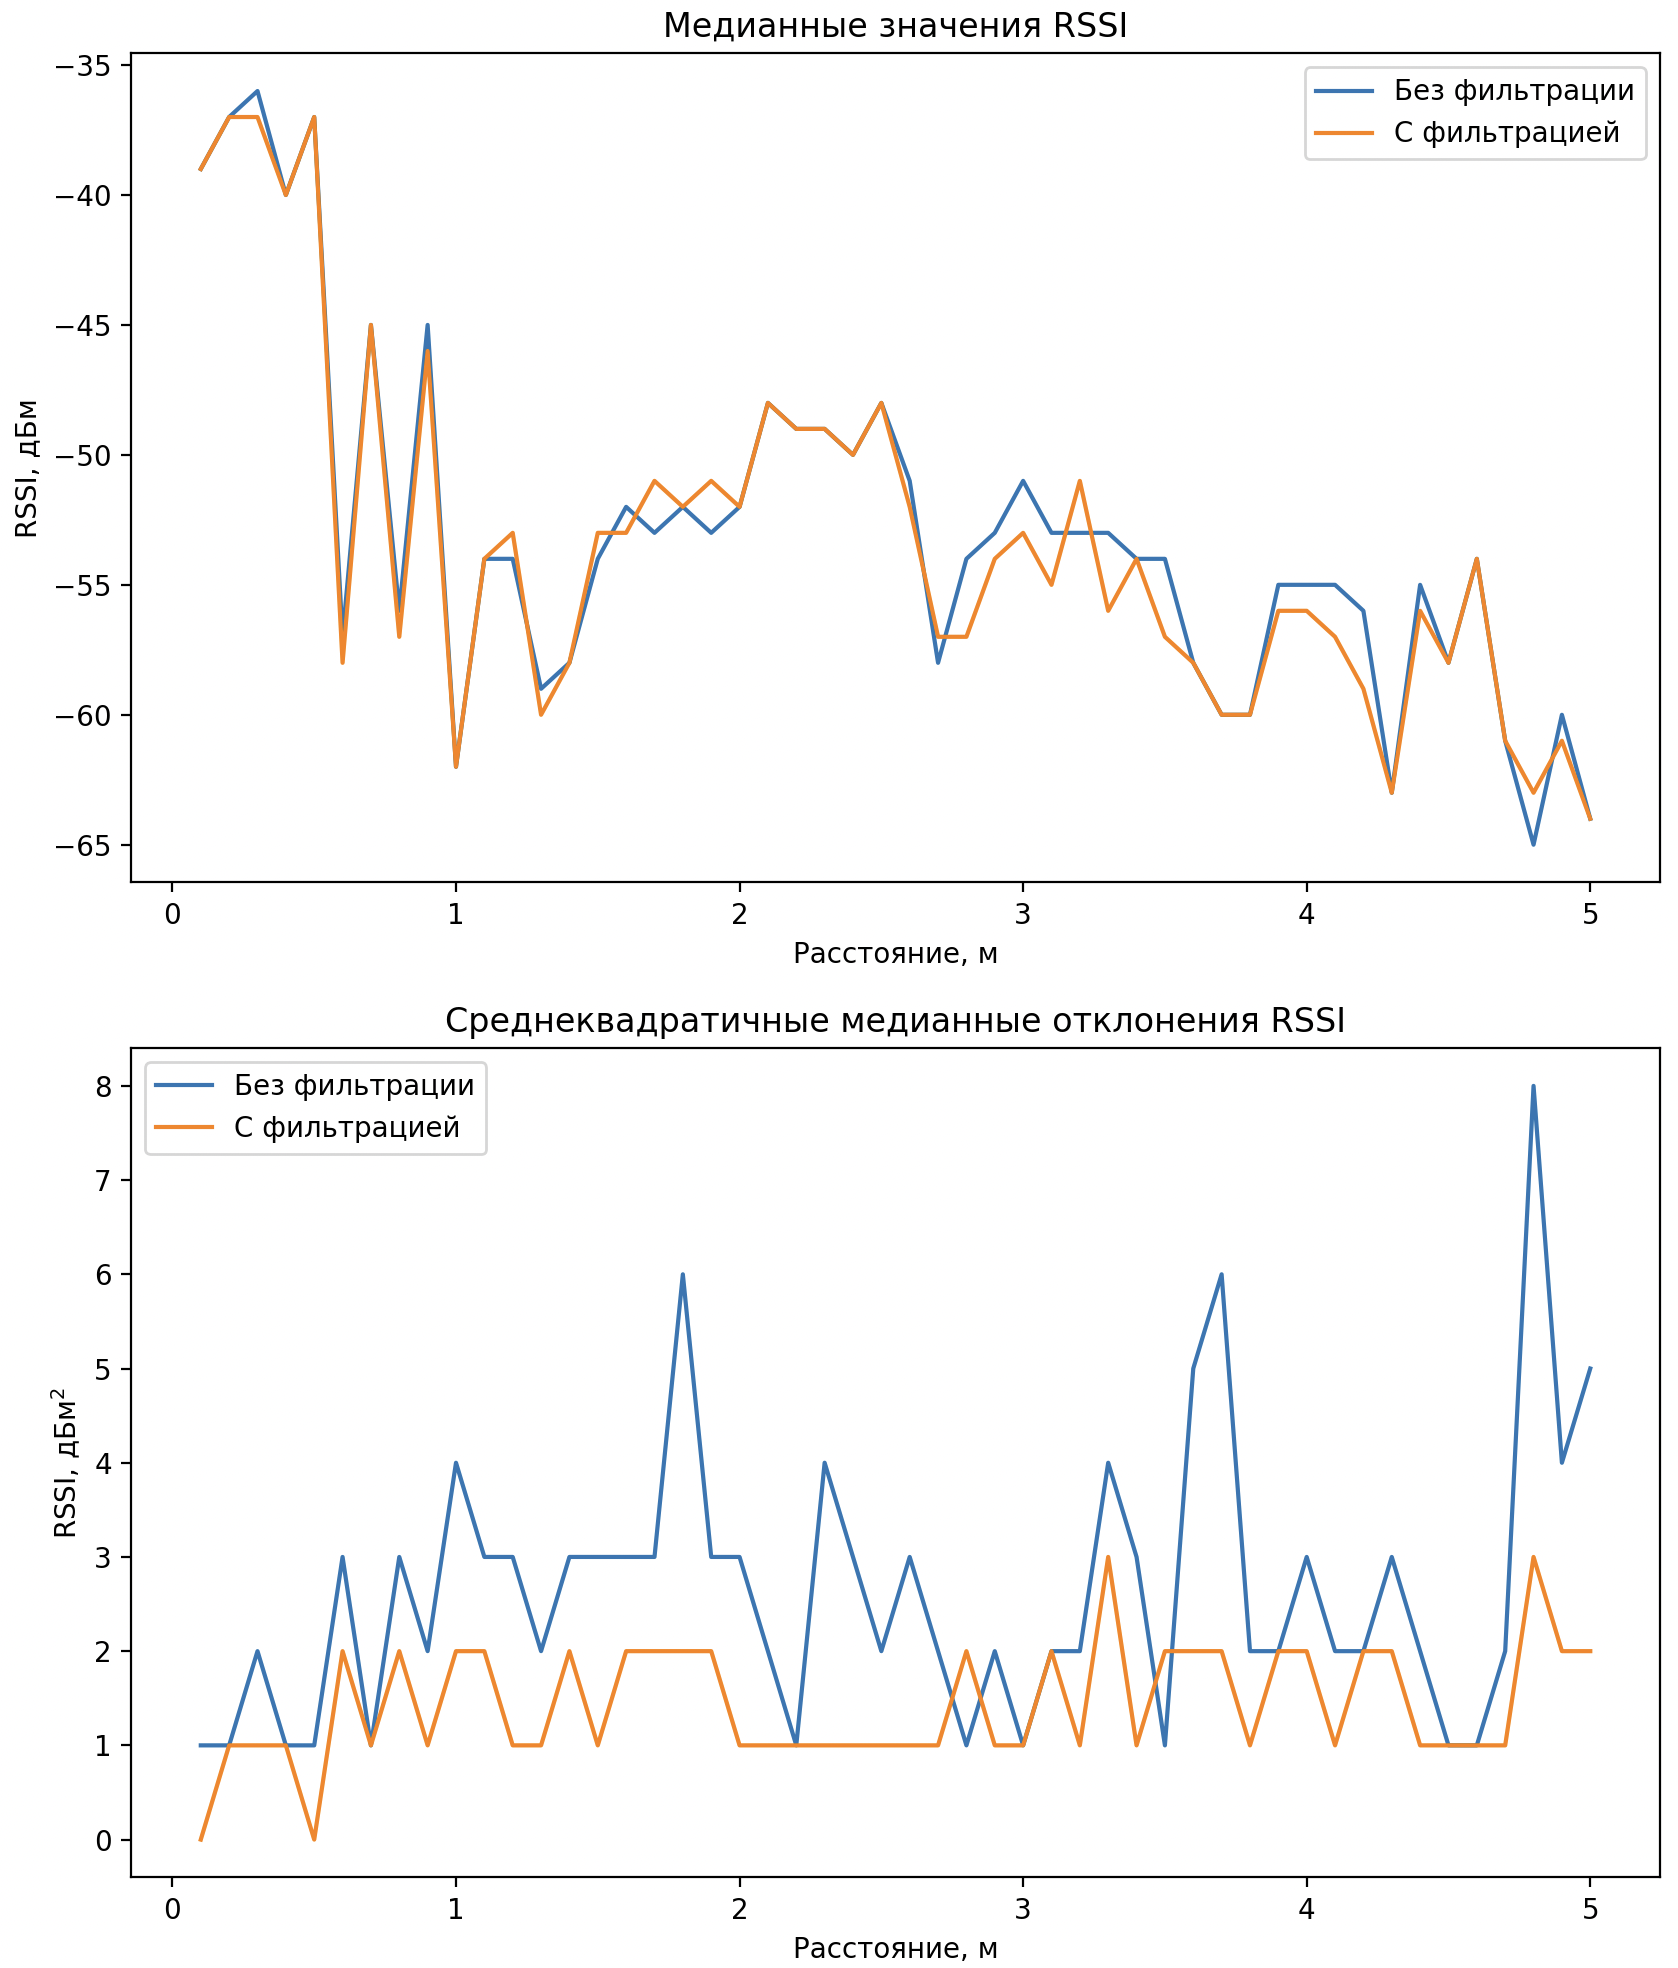
\includegraphics[width=\textwidth]{assets/medians.png}
	\caption{Сравнение медианных значений мощности сигнала до и после фильтрации}
	\label{fig:medians}
\end{figure}

\section{Обучение модели}

На рисунках \ref{fig:heatmap}-\ref{fig:hist-filtered} представлена визуализация оптимальной гауссовой смеси. Характеристики полученной модели:
\begin{itemize}[label*=---]
	\item Число компонент: 8;
	\item Значение метрики MSE при сравнении с исходным распределением: 0.0002907611;
	\item Отклонение коэффициента регрессии в модели потерь мощности сигнала на пути от источника до приёмника: 0.0058126679.
\end{itemize}

\begin{figure}[H]
	\centering
	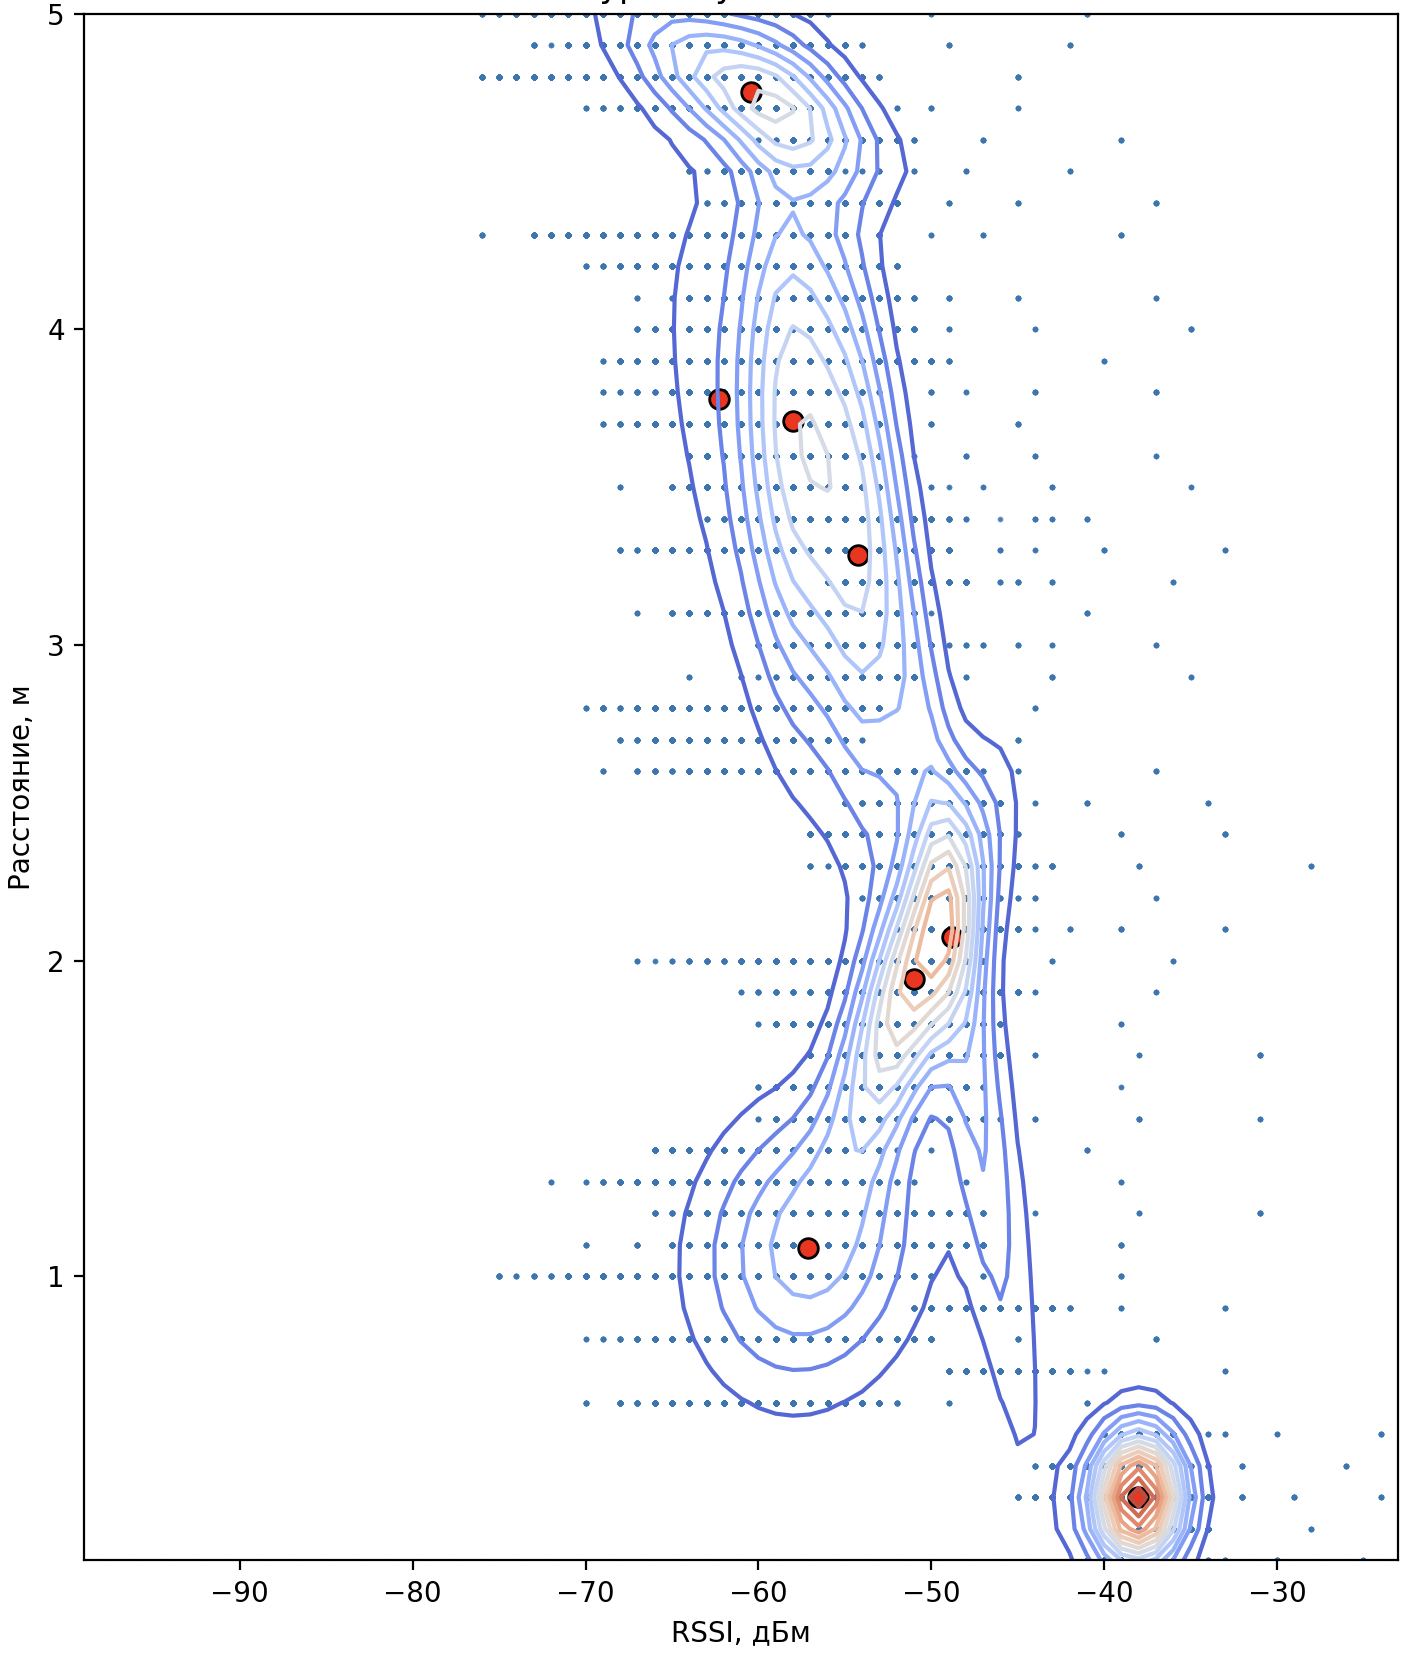
\includegraphics[width=\textwidth]{assets/deep.png}
	\caption{Контуры оптимальной гауссовой смеси}
	\label{fig:deep}
\end{figure}

\begin{figure}[H]
	\centering
	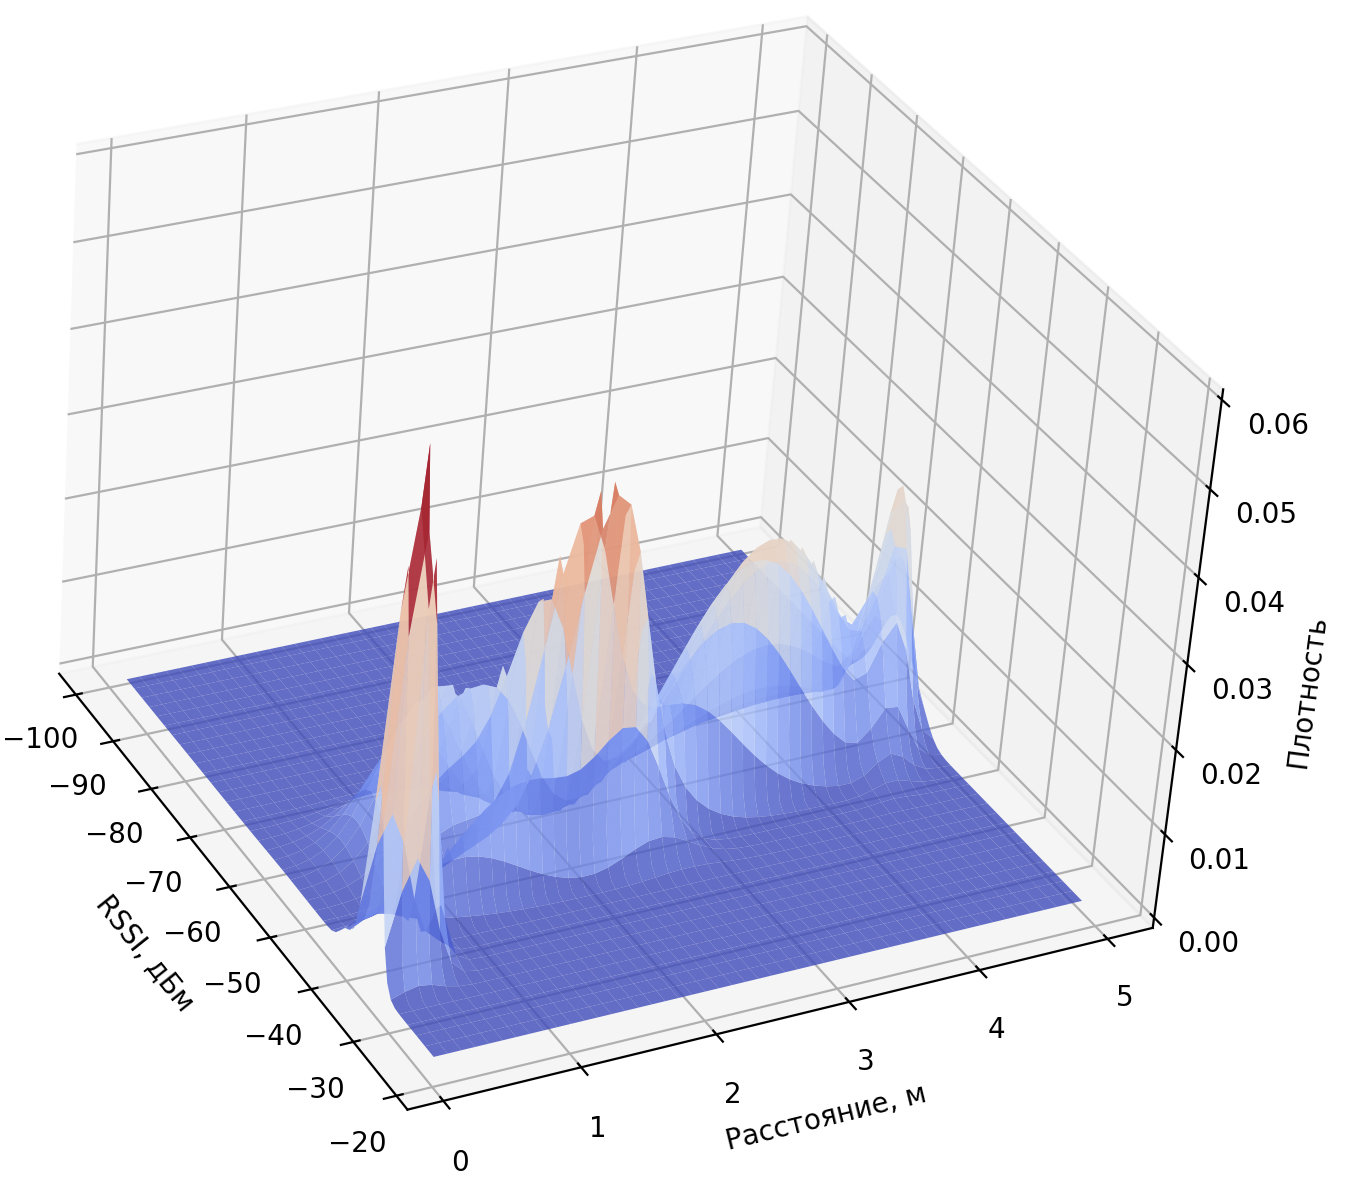
\includegraphics[width=\textwidth]{assets/gmm-hist.png}
	\caption{Гистограмма оптимальной гауссовой смеси}
	\label{fig:gmm-hist}
\end{figure}



\section{Вывод}

В данном разделе было проведено обучение модели гауссовой смеси и сравнение с исходным набором данных. В результате получилась модель из 8 компонент, значение метрики MSE составило 0.0002907611.


